%
\begin{isabellebody}%
\setisabellecontext{AMA{\isacharunderscore}possible}%
%
\isadelimtheory
%
\endisadelimtheory
%
\isatagtheory
%
\endisatagtheory
{\isafoldtheory}%
%
\isadelimtheory
%
\endisadelimtheory
%
\isadelimdocument
%
\endisadelimdocument
%
\isatagdocument
%
\isamarkupsection{Is Automated Kantian Ethics Possible?%
}
\isamarkuptrue%
%
\endisatagdocument
{\isafolddocument}%
%
\isadelimdocument
%
\endisadelimdocument
%
\begin{isamarkuptext}%
Many philosophers are averse to the idea that a computer could perform ethical 
reasoning or that the categorical imperative could provide an algorithm for
moral judgement. For example, Rawls asserts, ``it is a serious misconception to think of the CI-procedure 
as an algorithm intended to yield, more or less mechanically, a correct judgment. There is no such 
algorithm, and Kant knows this" \citep[166]{rawlslectures}. Ebels-Duggan also claims, ``no one supposes that the Categorical
Imperative provides a mechanical algorithm that delivers all by itself a complete account of what we 
ought to do in any given situation" \citep[174]{ebelsduggan}. However unmechanical ethical reasoning
may seem, these claims are not obvious and require further justification. After all, computers may eventually 
learn to simulate human mental activity entirely, as shown by progress in brain simulation \citep{brainsimulation}. 
Philosophers who believe that mental activity determines moral reasoning,\footnote{what's the name for these
guys? do they have a name?} must explain why computers can, in theory, simulate mental processes like arithmetic 
and language, but cannot perform ethical reasoning. Without a soul or God-based account of ethical reasoning, 
it is not obvious that it is theoretically impossible to automate ethical reasoning. 

In this section,
I explore potential arguments for why the categorical imperative could not be automated. When 
philosophers say that the categorical imperative is not an algorithm, they are often are gesturing to the complexity
of ethical judgement. They refer to the difficulty in determining morally relevant circumstances of a maxim or the common 
sense required for a computer to behave ethically as arguments against a categorical imperative ``algorithm." 
I will show in this section that these difficulties do not render automated Kantian ethics impossible, but 
merely difficult. There categorical imperative may not provide a simple and immediate algorithm, but, as
I demonstrate in this thesis, some parts of moral judgement using the FUL can be automated using not one
algorithm, but the many algorithms necessary to automatically prove logical theorems.

In \emph{Universal Laws and Ends In Themselves}, O'Neill presents an early account against the existence of an algorithm for
moral behavior. She points out that Kant draws an important distinction between a morally worthy maxim
and a morally worthy action: the latter requires a good will, motivated by duty. She argues that, 
``Kant defines duty not (as would be common today) as outward performance of a certain sort, but as action
that embodies a good will" \citep[345]{oneilluniversallaws}. Under this understanding of moral behavior, 
it seems unlikely that a computer could, in the near future, behave ``morally," since a computer does 
not have the same kinds of motivations and will as a human being. If a computer is not a fully rational
being, then, it is not the kind of thing that can behave morally.

The idea that, under Kant's account, a computer cannot behave morally, does not preclude the kind 
of automated categorical imperative test that I present in this thesis. O'Neill argues that the FUL
serves as a test of morally worthy maxims, and an automated categorical imperative test can be used 
to identify this kind of maxim. Perhaps a computer cannot act on a morally relevant maxim from a motivation of duty, 
but it certainly can act on this maxim nonetheless. For example, a self-driving car can choose to swerve to hit a tree
to avoid injuring pedestrians in the crosswalk. This action may be one that acts on a morally worthy maxim
\emph{even if} the self-driving car is not motivated by duty. The discpline of machine ethics is partially
spurred by the recognition that, as automated agents become more powerful, they will need to make
morally consequential decisions. Automated agents may be incapable of moral behavior, but automated agents that mimic
moral behavior are surely better than agents that ignore morality entirely. Moreover, this argument
has no bearing on the possibility of computational ethics, as evaluating the moral status of a maxim can 
help philosophers study Kantian ethics even if the computer performing the evaluation is incapable of 
moral behavior.

Another challenge for automated Kantian ethics identified by O'Neill is that the FUL test requires that
a maxim be given as input. O'Neill notes that the test assumes ``that agents will have certain tentative 
plans, proposals and policies which they can consider, revise or reject or endorse and pursue" \citep[343]{oneilluniversallaws}.
Kant even claims that the difficulty of determining an agent's potential maxim, which is their
own, subjective understanding of their principle of action, is a reason that we may never be able 
to know if morally worthy action has been performed \cite[345]{oneilluniversallaws}. 

The challenge of mapping actions to maxims is a limitation of my system, but it is not insurmountable. In Section Upshot,
I argue that, before my system can be used in practice, it must be paired with an ``input parser," that can
translate choices that an automated agent faces into maxims in a logic that my system can
evaluate. This limitation directly follows from the difficulty in mapping a potential action
to the maxim of action, whether concerning human action or machine action. As argued in Section Upshot,  
this is not an insurmountable obstacle for automated ethics. Future work could develop heuristics to 
map actions to maxims, perhaps by extracting the circumstances, act, and goal. Moreover, proponents of the 
human-in-the-loop model may argue that the solution to this problem is to have a human being manually create
such mappings, either dynamically or in a cached manner. Given that determining the maxim of action is a challenge
for human Kantian ethical reasoners, it is unsurprising that it is a major hurdle for automated Kantian agents. 
Computational ethics remains unaffected by this concern because philosophers often debate 
the morality of specific maxims or metaethical properties of the categorical imperative, all of which can
be studied without an algorithm for parsing moral dilemmas into the relevant maxims.

As one of the strongest arguments against a categorical imperative algorithm, O'Neill argues that 
the FUL is not supposed to provide a mechanism for deriving all morally worthy maxims from scratch. She notes
that ``we usually already have learnt or worked out the moral standing of many common maxims of duty," 
and so approach moral deliberation with an ``almanac" of morally worthy and empty maxims \citep[394]{oneilluniversallaws}. Rational agents
navigating the world rarely recalculate the moral status of each potential maxim of action; instead, we consult our
almanac of maxims. The categorical imperative is useful to verify the rightness or 
wrongness of a maxim, but is not part of the bulk of human ethical reasoning.

While human beings cannot repeatedly apply the universalizability test to all potential maxims during 
every moral dilemma, computers have the computational power to do so. Human beings are 
equipped with enough prior knowledge or ``common sense" to have an almanac of morally worthy maxims,
but we have limited computational power. Computers, on the other hand, are comparatively
much more capable of computation and thus can repeatedly recompute the results of the categorical
imperative test. They do not come equipped with an almanac of maxims, but can simply recompute this
almanac every time they need to make a decision. Human beings use common sense to make up for their computational
limitations, and automated moral agents can use computational power to reduce the need for common sense.

Daniela Tafani takes this argument one step further by arguing that this ``alamnac" of maxims already 
includes the moral status of the maxims in questions; human beings already
know which maxims are morally worthy and which are morally lacking. The categorical imperative test
merely reminds us, in moments of weakness, when we are tempted to make an exception to the moral law for 
our own convenience or pleasure, that the moral law has no exceptions \citep[9]{tafani}. Thus, she claims
that ``the Kantian test is therefore as useless for machines as it is for anyone who does
not already know what to do" \citep[8]{tafani}.\footnote{Translated from the original paper using Google Translate.} 
Understanding the categorical imperative test as a reminder
instead of a derivation tool also explains a fact noted by \cite{constofreason} that I discuss in Section Applications as a 
response to the tailoring objection: the FUL cannot handle bad-faith attempts to generate false
positives or negatives. The test only returns the right result when an agent sincerely attempts to 
represent their maxim of action, not when an adversary attempts to ``trick" the categorical imperative.%
\end{isamarkuptext}\isamarkuptrue%
%
\begin{figure}
\centering
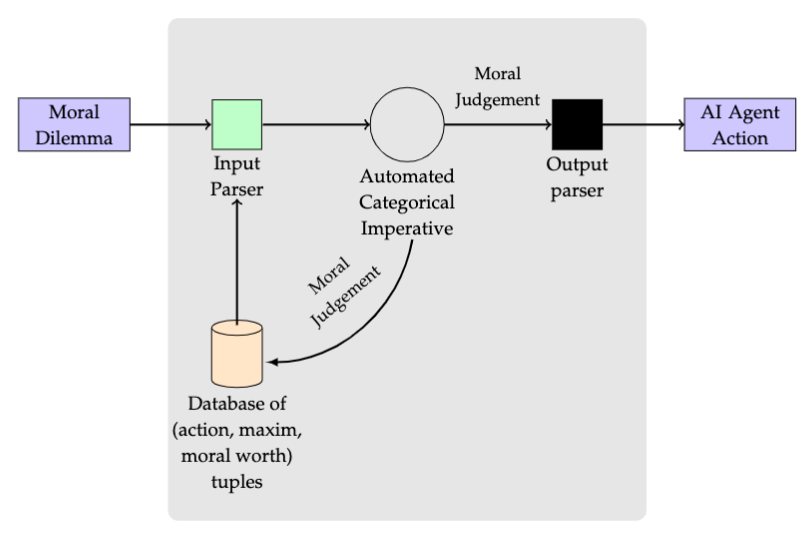
\includegraphics[scale=0.5]{inputparser.png}
\caption{A refined version of Figure \ref{fig:AIengine} in which the input parser learns from a database
of action-maxim mappings, which is in turn fed the output of my automated Kantian ethics system. } \label{fig:inputparser}
\end{figure}
%
\begin{isamarkuptext}%
This understanding of the role of the categorical imperative not only fails to render automate moral
reasoning impossible, but it also offers insight into how to solve the challenge of creating an input parser.
If the categorical imperative test is only useful to those who have some prior moral knowledge, then prior moral
knowledge should be used to create an input parser. Specifically, some kind of machine learning-based approach
could learn action-maxim mappings from a database of such mappings compiled by a human being. Moreover, 
the human being could assign each maxim in the database a rightness or wrongness score. My implementation
of the automated categorical imperative would then simply check the work of this machine learning algorithm and transform
a fuzzy prediction into a provable, rigorous moral judgement. Moreover, this rigorous moral judgement
could in turn be fed into the database of maxims to make the intput parser smarter. One example of 
this kind of system is shown in Figure \ref{fig:inputparser}. The combination of 
prior knowledge of some maxims' moral worth and the ability of a computer to constantly perform the
universalizability test could not only match human ethical reasoning but perhaps also surpass it
by double checking the moral intuitions that we take for granted. A computer with no common sense or prior knowledge
may indeed be unable to reason using the categorical imperative, but one equipped with some prior knowledge
of maxims and their moral worth may even help us better reason about morality.%
\end{isamarkuptext}\isamarkuptrue%
%
\isadelimtheory
%
\endisadelimtheory
%
\isatagtheory
%
\endisatagtheory
{\isafoldtheory}%
%
\isadelimtheory
%
\endisadelimtheory
%
\end{isabellebody}%
\endinput
%:%file=~/Desktop/cs91r/paper/AMA_possible.thy%:%
%:%24=6%:%
%:%36=8%:%
%:%37=9%:%
%:%38=10%:%
%:%39=11%:%
%:%40=12%:%
%:%41=13%:%
%:%42=14%:%
%:%43=15%:%
%:%44=16%:%
%:%45=17%:%
%:%46=18%:%
%:%47=19%:%
%:%48=20%:%
%:%49=21%:%
%:%50=22%:%
%:%51=23%:%
%:%52=24%:%
%:%53=25%:%
%:%54=26%:%
%:%55=27%:%
%:%56=28%:%
%:%57=29%:%
%:%58=30%:%
%:%59=31%:%
%:%60=32%:%
%:%61=33%:%
%:%62=34%:%
%:%63=35%:%
%:%64=36%:%
%:%65=37%:%
%:%66=38%:%
%:%67=39%:%
%:%68=40%:%
%:%69=41%:%
%:%70=42%:%
%:%71=43%:%
%:%72=44%:%
%:%73=45%:%
%:%74=46%:%
%:%75=47%:%
%:%76=48%:%
%:%77=49%:%
%:%78=50%:%
%:%79=51%:%
%:%80=52%:%
%:%81=53%:%
%:%82=54%:%
%:%83=55%:%
%:%84=56%:%
%:%85=57%:%
%:%86=58%:%
%:%87=59%:%
%:%88=60%:%
%:%89=61%:%
%:%90=62%:%
%:%91=63%:%
%:%92=64%:%
%:%93=65%:%
%:%94=66%:%
%:%95=67%:%
%:%96=68%:%
%:%97=69%:%
%:%98=70%:%
%:%99=71%:%
%:%100=72%:%
%:%101=73%:%
%:%102=74%:%
%:%103=75%:%
%:%104=76%:%
%:%105=77%:%
%:%106=78%:%
%:%107=79%:%
%:%108=80%:%
%:%109=81%:%
%:%110=82%:%
%:%111=83%:%
%:%112=84%:%
%:%113=85%:%
%:%114=86%:%
%:%115=87%:%
%:%116=88%:%
%:%117=89%:%
%:%118=90%:%
%:%119=91%:%
%:%120=92%:%
%:%121=93%:%
%:%122=94%:%
%:%123=95%:%
%:%124=96%:%
%:%125=97%:%
%:%126=98%:%
%:%127=99%:%
%:%128=100%:%
%:%129=101%:%
%:%130=102%:%
%:%131=103%:%
%:%132=104%:%
%:%135=107%:%
%:%136=108%:%
%:%137=109%:%
%:%138=110%:%
%:%139=111%:%
%:%140=112%:%
%:%143=114%:%
%:%144=115%:%
%:%145=116%:%
%:%146=117%:%
%:%147=118%:%
%:%148=119%:%
%:%149=120%:%
%:%150=121%:%
%:%151=122%:%
%:%152=123%:%
%:%153=124%:%
%:%154=125%:%
%:%155=126%:%
%:%156=127%:%
%:%157=128%:%